%%
%% SIGMOD 2025 — New version following PRM writing style
%%
\documentclass[sigconf]{acmart}

\AtBeginDocument{%
  \providecommand\BibTeX{{Bib\TeX}}}

\setcopyright{acmlicensed}
\copyrightyear{2025}
\acmYear{2025}
\acmDOI{XXXXXXX.XXXXXXX}
\acmConference[SIGMOD '25]{ACM International Conference on Management of Data}{June 2025}{Berlin, Germany}
\acmISBN{978-1-4503-XXXX-X/2025/06}

%%\usepackage[utf8]{inputenc}
%%\usepackage[T1]{fontenc}
%\usepackage{amsmath}
%\usepackage{amsfonts}
%%\usepackage{amssymb}
%\usepackage{booktabs}
%\usepackage{graphicx}
%\usepackage{microtype}
%\usepackage{xcolor}
%\usepackage{algorithm}
%\usepackage{algpseudocode}
%\usepackage{enumitem}
\usepackage{hyperref}       % hyperlinks
\usepackage{url}            % simple URL typesetting
\usepackage{booktabs}       % professional-quality tables
\usepackage{amsfonts}       % blackboard math symbols
\usepackage{nicefrac}       % compact symbols for 1/2, etc.
\usepackage{microtype}      % microtypography
\usepackage{xcolor}         % colors
\usepackage{amsmath,dsfont}
\usepackage{algorithm}
\usepackage{algpseudocode}
\usepackage{graphicx}
\usepackage{colortbl}
\usepackage{wrapfig}
\usepackage{balance}
\usepackage{enumitem}
%% Handy shorthands
\newcommand{\CIMRIS}{\textsc{CIM-RIS}}
\newcommand{\pa}{p_u^a}
\newcommand{\pd}{p_u^d}
\newcommand{\pt}{p_u^t}
\newcommand{\sig}{\sigma}
\newcommand{\E}{\mathbb{E}}
\newcommand{\C}{\mathbb{C}}
\newcommand{\I}{\mathbb{I}}
\newcommand{\P}{\mathbb{P}}

\begin{document}

\title{Coupon influence maximization under random walk diffusion in social network}

\author{Anonymous Author(s)}

\renewcommand{\shortauthors}{Anon.}

%% ============================================================
%% ABSTRACT
%% ============================================================
\begin{abstract}

  

\end{abstract}

\begin{CCSXML}
<ccs2012>
 <concept>
  <concept_id>10002951.10002952.10002953.10010820</concept_id>
  <concept_desc>Information systems~Social networks</concept_desc>
  <concept_significance>500</concept_significance>
 </concept>
 <concept>
  <concept_id>10003752.10003809.10010170.10010171</concept_id>
  <concept_desc>Theory of computation~Approximation algorithms analysis</concept_desc>
  <concept_significance>300</concept_significance>
 </concept>
</ccs2012>
\end{CCSXML}

\ccsdesc[500]{Information systems~Social networks}
\ccsdesc[300]{Theory of computation~Approximation algorithms analysis}

\keywords{influence maximization, coupon diffusion, random walk,
          reverse influence sampling, submodular optimization}

\maketitle

%% ============================================================
%% 1. INTRODUCTION
%% ============================================================
\section{Introduction}
\label{sec:intro}

Word-of-mouth and viral marketing have become important strategies for
product promotion in social networks.
By selecting a small set of influential seed users, a company can
promote products' adoption by word-of-mouth marketing along social connections.
However, how to choose the best initial seed users is a challenge,
 a problem commonly referred
to as influence maximization (IM)~\cite{kempe2003maximizing}.
Over the past two decades, IM has been extensively studied under
classical models such as the Independent Cascade (IC) and Linear
Threshold (LT) models, where activated nodes attempt to trigger their
neighbors in a broadcast manner, i.e.,one node could trigger multiple neighbors~\cite{domingos2001mining,borgs2014maximizing,tang2015influence}.
However, many real-world promotional campaigns deviate from this
paradigm.
For example, a company sends some digital coupons for product promotion in the online social network (e.g., Social Media Promo Code from Amazon, Percentage Off from various e-commerce platforms,
promotion codes form Google Play). The diffusion model of digital coupons is quite  different from the classical IM: A digital coupon could only be passed from one user to only one neighbor, where the diffusion follows random walk-like mechanism rather than IM's broadcast manner. Once a digital coupon is consumed by a user, the coupon cannot be further transferred in the social network. A user who consumes at least one coupon could be treated as activated. The aim is  to activate as more as possible users for future potential consumption. However, since a user might consume multiple coupons, how to choose the best initial seed users to activate most final users is a challenge, which we define as coupon influence maximization(CIM for short). Though IM has been well studied, the solution to IM could not be explicitly applied to CIM, because of the different underlying  diffusion mechanism. \textcolor[rgb]{1.00,0.00,0.00}{$However$}, the CIM is rarely investigated in previous works.



We consider a concrete example:
A company wants to promote a new product and issues $k$ digital coupons of Percentage off
to $k$ seed users. We first consider the diffusion of one coupon. When a user receives the coupon, he/she has three candidate actions: consuming action, dropping action, and transferring action. For the consuming action, if the user didn't consume coupons previously, he/she consumes the coupon and becomes to activation state; if the user has consume other coupons previously, he/she keeps in the activation state, i.e., we allow the consumption of multiple coupons. After the consuming action, the diffusion of the coupon terminates at the user.
 For the dropping action, the user refuses to consume\&transfer the coupon, and the user keep its state unchanged. Meanwhile, the diffusion of the coupon terminates at the user.
 For the transferring action, the user refuse to consume\&drop the coupon, and transfer the coupon to only one random neighbor. Meanwhile, the user keep its state unchanged. The coupon diffuses in the social network following the above mechanism until termination. We now turn to the diffusion of multiple coupons: each coupon follows the same diffusion mechanism introduced above.
  For simplification, we assume that different coupon diffuses independently. Hence, a user may consume multiple coupons, but only be counted as one activated user. Note that the users who only transfer coupons, but do not consume any coupon, are counted as inactive. 
 When the diffusion of all coupons terminates, we count the activated users. 
The primary objective is to select $k$ seed nodes that maximize the
expected number of final activated nodes. Inappropriate seed nodes would lead to either the scenario that one user consume too many coupons, or the scenario that too many coupons are dropped. Hence, the CIM problem is a parallel important problem of IM. However, we still lack a strict analysis of CIM and the solution to the problem.

In the paper, we propose the strict formalism of the CIM problem. We investigate the influence of network structure on CIM and prove that CIM problem is NP-hard. We further analytically shown that 
the objective function(expected number of activated users) is monotone and submodular. Based on the NP-hard and submodular properties,  a plausible solution is greedy algorithm. The IM algorithm first samples RR sets and transfers IM problem into set covering problem, based on which greedy algorithm is performed. Inspired by the process, we first provide the special generation process for RR sets based on the diffusion mechanism of CIM. We then demonstrate that the induced set covering problem of CIM is quite different from IM. We then propose a dedicated greedy algorithm for the induced set cover problem of CIM. We prove that our algorithm could reach an approximation ratio $1-1/e$ and has time complexity \textcolor[rgb]{1.00,0.00,0.00}{$xxxx$}. At last, Experiments in various datasets demonstrate the effectiveness and efficiency of our algorithm. 

An important point of our study is that coupon influence maximization is
completely different from classical IM:
(a) The diffusion mechanism is different. In classical IM, the information spreads in a broadcast manner, where one user could trigger multiple neighbors. However, in CIM, the information spreads in a random walk-like manner, where one user could only transfer to at most one neighbor(or consume/drop it). Moreover, the users that only transfer information(not consume information) are treated inactive in CIM, whereas all users on a spreading path are treated active. (b) In the solution algorithm, the RR set generation process and the induced set cover problem of CIM is more complex than these of IM. 
We design a dedicated RR set generation process and the corresponding greedy algorithm for CIM.


In summary, our contributions are as follows.
First, we initiate the formal study of coupon influence maximization by
proposing the coupon influence model, which captures the single-copy,
multi-coupon nature of real-world coupon campaigns, and by defining two
campaign objectives: adoption-spread maximization and coupon
usage-rate maximization.
Second, we prove that CIM is NP-hard and show that the adoption spread
function is monotone and submodular under the seed-node and coupon-index
representation.
Third, we develop a tailored reverse influence sampling scheme based on
$k$-joint RR sets and build the \CIMRIS{} algorithm for scalable seed
selection.


%% ============================================================
%% 2. RELATED WORK
%% ============================================================
\section{Related Work}
\label{sec:related}

%% ============================================================
%% 3. MODEL AND PROBLEM DEFINITION
%% ============================================================
\section{Problem Definition}
\label{sec:model}

Let $G=(V,E)$ be a directed graph with $n = |V|$ nodes and $m = |E|$ edges, where each node $v\in V$ represents a user and each directed edge $(u,v)\in E$ represents the connection between users. Each edge $(u,v)\in E$ is associated with a weight $p(u,v)$.Given a subset of nodes $S\subseteq V$ with $|S| = k$, denoted as the initial seed set, we consider the following propagation process $\mathbb{C}$:

\begin{itemize}
\item
Initially, the $k$ seed nodes in $S$ each hold one coupon and begin propagating.

\item
When a coupon arrives at a node $u$, the node takes one of three actions: it consumes the coupon with probability $p_u^a$, drops the coupon with probability $p_u^d$, or transfers the coupon with probability $p_u^t$, where $p_u^a + p_u^d + p_u^t = 1$.

\item
If $u$ consumes the coupon, it is counted as an activated user and the diffusion of the coupon terminates. If $u$ drops the coupon, the diffusion of the coupon also terminates. Otherwise, $u$ transfers the coupon to one of its out-neighbors chosen at random according to $p(u,v)$, satisfying
$p(u,v)\ge0$,
$\sum_{v\in N^+(u)} p(u,v)=1$, whenever $N^+(u)\neq \emptyset$.

\item
The coupon follows the above diffusion mechanism until termination.

\end{itemize}

Transferring alone yields no consumption benefit; only consumption counts a user as activated. Each coupon is non-duplicable, and at any time it is held by at most one user. For the same coupon, the behavior of each node is sampled independently across coupon visits. We assume that there exists a constant \(\epsilon>0\) such that \(p_u^a+p_u^d\ge \epsilon\) for every \(u\in V\), which guarantees that every coupon terminates almost surely.

Different coupons propagate independently and do not interfere with one another. In particular, the propagation of one coupon does not block another coupon or alter the action probabilities of any user. A user may therefore consume multiple coupons, but is counted only once in the final number of activated users. Users who only transfer coupons but never consume any coupon are regarded as inactive.

For a single coupon seeded at $s$, let $q_{s,u}$ denote the probability that this coupon is eventually consumed by user $u$.Because different coupons propagate independently, the probability that a user $u$ consumes at least one of the coupons issued by $S$ is
\begin{equation}
\Pr[\text{$u$ consumes some coupon}] = 1-\prod_{s\in S}\bigl(1-q_{s,u}\bigr).
\end{equation}
We define the spread of $S$ as the expected number of distinct users who consume at least one coupon:
\begin{equation}
\sigma(S) = \sum_{u \in V} \Bigl(1-\prod_{s\in S}\bigl(1-q_{s,u}\bigr)\Bigr).
\end{equation}
This objective measures the number of distinct consuming users and counts each user at most once, even if the user consumes multiple coupons.

\textcolor[rgb]{1.00,0.00,0.00}{For comparison, one may also maximize the total number of consumed coupons $\rho(S)$ (or, equivalently, the usage rate $\rho(S)/k$) when the organizer mainly cares about how many issued coupons are used.}



\begin{definition}[CIM: Spread Maximization]
\label{def:cim}
Given a graph $G$, node behavior parameters $\{(p_u^a,p_u^d,p_u^t)\}_{u\in V}$, and a coupon budget $k$, the Coupon Influence Maximization (CIM) aims to find an optimal seed set $S^*$ such that the spread $\sigma(S^*)$ is maximized, i.e.,
\begin{equation}
S^{*} = \arg\max_{S \subseteq V,\ |S|=k}\; \sigma(S).
\end{equation}
\end{definition}
\textbf{Challenge}.For the spread objective, simply selecting the $k$ nodes with the largest individual spreading potential may be suboptimal, since different coupons may end at the same consuming user, which is only counted once in $\sigma(S)$. Moreover, although the objective is to increase distinct consumers, the problem is still tightly related to forwarding paths, because a coupon can be consumed only after it reaches the user through a single-path walk. Therefore, CIM is non-trivial both in considering overlap among multiple coupons and in considering the relationship between reachability and consumption.



%% ============================================================
%% 4. THEORETICAL ANALYSIS
%% ============================================================
\section{Theoretical Analysis}
\label{sec:theory}

We establish the computational hardness of CIM and the structural
properties of its expected spread. Throughout this section, we use the
independent coupon walks defined in Section~\ref{sec:model}: each seed
receives one coupon, and users may consume multiple coupons while being
counted only once.

\begin{theorem}
\label{thm:nphard}
CIM is NP-hard, even on two-layer directed acyclic graphs.
\end{theorem}

\begin{proof}[Proof sketch]
We reduce from vertex cover in cubic graphs~\cite{garey1976simplified}.
Given a cubic graph $H=(V_H,E_H)$ and a budget $K$, create a node $a_x$
for each vertex $x$ and a node $b_e$ for each edge $e$, with arcs
$a_x\to b_e$ for incident pairs. Set the behavior probabilities
$(p^a,p^d,p^t)$ to $(1/2,0,1/2)$ at $a_x$ and $(1/4,3/4,0)$ at $b_e$;
each $a_x$ chooses uniformly among its three out-neighbors.
All nodes are eligible seeds. Replacing a selected $b_e$ with an
unselected $a_x$ loses at most $1/4$ in expected spread and gains at
least $1/2$, so every optimum selects only $a_x$ nodes.
For $K$ such seeds, let $n_0$ count the uncovered edges of $H$. Then
\[
  \sigma(S)=\frac{K}{2}+\frac{3K}{24}
             -\frac{3K-|E_H|+n_0}{576}.
\]
The value reaches $B=K/2+3K/24-(3K-|E_H|)/576$ if and only if
$n_0=0$. Thus the threshold is attainable exactly when $H$ has a
vertex cover of size at most $K$. The complete construction and both
directions of the reduction appear in Appendix~\ref{app:hardness}.
\end{proof}

Next, extend the expression for $\sigma(S)$ in
Section~\ref{sec:model} to every $S\subseteq V$; the budget $k$
constrains the optimization, rather than the domain of the function.
For $v\notin S$, write
$\Delta(v\mid S)=\sigma(S\cup\{v\})-\sigma(S)$.

\begin{theorem}
\label{thm:monosub}
The expected spread $\sigma:2^V\to\mathbb{R}_{\geq 0}$ is normalized,
monotone, and submodular.
\end{theorem}

\begin{proof}
By independence across coupons, the single-coupon probabilities
$q_{s,u}$ do not depend on the other seeds. Hence
\begin{equation}
\label{eq:seed-marginal}
  \Delta(v\mid S)
    =\sum_{u\in V}q_{v,u}\prod_{s\in S}(1-q_{s,u}).
\end{equation}
The empty-product convention gives $\sigma(\varnothing)=0$.
Since $q_{s,u}\in[0,1]$, every summand in
\eqref{eq:seed-marginal} is nonnegative, proving monotonicity.
For $S\subseteq T\subseteq V$ and $v\notin T$, we have
\[
  \prod_{s\in S}(1-q_{s,u})
    \geq\prod_{s\in T}(1-q_{s,u})
  \qquad\text{for every }u\in V.
\]
Multiplying by $q_{v,u}$ and summing over $u$ yields
$\Delta(v\mid S)\geq\Delta(v\mid T)$, which proves submodularity.
\end{proof}

The diminishing returns arise from overlap among the eventual
consumers of independent coupons. They do not require users to change
their behavior after consuming a coupon.

\begin{corollary}
\label{cor:exact-greedy}
For $1\leq k\leq n$, let $S_{\mathrm{gr}}$ be the set obtained by
starting from $\varnothing$ and repeatedly adding an unselected node
with the largest exact marginal gain. Then
\[
  \sigma(S_{\mathrm{gr}})
    \geq\left[1-\left(1-\frac{1}{k}\right)^k\right]\sigma(S^*)
    \geq(1-1/e)\sigma(S^*).
\]
\end{corollary}

This follows from Theorem~\ref{thm:monosub} and the classical greedy
bound under a cardinality constraint~\cite{nemhauser1978analysis}.
The corollary concerns exact marginal gains; a sampling-based
implementation additionally requires a valid estimator and an analysis
of its estimation error.

The hardness lies in seed selection, while the single-coupon
probabilities can be computed by linear algebra. Define
$T_{uv}=p_u^t p(u,v)$ on edges and $T_{uv}=0$ otherwise, with
$p_u^t=0$ at nodes without out-neighbors. Let
$D_a=\operatorname{diag}((p_u^a)_{u\in V})$ and $Q=(q_{s,u})$.
Conditioning on the first action gives
\begin{equation}
\label{eq:single-coupon-kernel}
  Q=D_a+TQ,\qquad Q=(I-T)^{-1}D_a.
\end{equation}
The termination assumption implies $\|T\|_\infty\leq1-\epsilon<1$,
so the inverse exists. A dense computation of $Q$ requires $O(n^3)$
arithmetic operations and $O(n^2)$ storage. Once $Q$ is available,
maintaining the products in \eqref{eq:seed-marginal} gives a direct
greedy implementation using $O(kn^2)$ further arithmetic operations.
The cost of forming and storing $Q$ motivates estimating marginal
gains without materializing the full matrix, as pursued in
Section~\ref{sec:algo}.

%% ============================================================
%% 5. ALGORITHM: CIM-RIS
%% ============================================================
\section{Algorithm: \CIMRIS{}}
\label{sec:algo}

We construct an unbiased coverage estimator for the independent coupon
walks of Section~\ref{sec:model} and optimize it over seed sets
$S\subseteq V$ with $|S|=k$. The sampling unit contains one independent
hypothetical coupon walk from each candidate seed. Restricting these
walks to any fixed $S$ reproduces the joint distribution of its $k$
coupons. We group the sampled outcomes by consuming user to obtain
reverse sets and apply greedy maximum coverage directly on $V$.
This construction generates reverse sets by forward simulation and
inversion; it does not assume that a local backward traversal can
sample them. Its sampling cost is accounted for explicitly below.

\subsection{Reverse Sets for Independent Coupon Walks}

For each sample index $t$ and candidate seed $s\in V$, independently
simulate one coupon according to Section~\ref{sec:model}. Let
$Z_s^{(t)}\in V\cup\{\bot\}$ denote its eventual consumer, with
$\bot$ indicating discard. Thus
\begin{equation}
\label{eq:endpoint-law}
  \Pr[Z_s^{(t)}=u]=q_{s,u},\qquad
  \Pr[Z_s^{(t)}=\bot]=1-\sum_{u\in V}q_{s,u}.
\end{equation}
All action draws are independent across visits, candidate seeds, and
sample indices. In particular, two walks that visit the same node do
not share its action draw. The walks for unselected candidates are
hypothetical samples; the campaign still issues only $k$ coupons.

\begin{definition}[Reverse set of sampled consumers]
For a user $u\in V$ and sample index $t$, define
\[
  R_t(u)=\{s\in V:Z_s^{(t)}=u\}.
\]
One sample consists of the family $\mathcal{R}_t=(R_t(u))_{u\in V}$.
\end{definition}

These reverse sets record which candidate seeds have the same sampled
consumer. Each candidate belongs to at most one set in a family,
since its coupon has at most one consumer. The sets are not defined by
a shared graph with one fixed live edge per node.

\begin{lemma}[Coverage identity]
\label{lem:coverage}
For every fixed $S\subseteq V$ and $u\in V$,
\begin{equation}
\label{eq:reverse-coverage}
  \Pr[S\cap R_t(u)\ne\varnothing]
    =1-\prod_{s\in S}(1-q_{s,u}).
\end{equation}
\end{lemma}

\begin{proof}
By definition, $S\cap R_t(u)=\varnothing$ if and only if
$Z_s^{(t)}\ne u$ for all $s\in S$. Independence across candidate
seeds and \eqref{eq:endpoint-law} give probability
$\prod_{s\in S}(1-q_{s,u})$ for this event. Taking its complement
proves the claim. Thus the selected walks have exactly the independent
coupon-consumption probabilities specified in Section~\ref{sec:model}.
\end{proof}

Define the number of covered users in sample $t$ by
\[
  Y_t(S)=\sum_{u\in V}\I[S\cap R_t(u)\ne\varnothing].
\]
For $|S|=k$, $0\leq Y_t(S)\leq k$, since each selected walk consumes
at most one coupon. Draw $\theta$ independent sample families and set
\begin{equation}
\label{eq:empirical-spread}
  \hat{\sigma}_{\theta}(S)=\frac1\theta\sum_{t=1}^{\theta}Y_t(S).
\end{equation}

\begin{lemma}[Unbiasedness]
\label{lem:unbiased}
For every fixed seed set $S$,
$\E[\hat{\sigma}_{\theta}(S)]=\sigma(S)$.
\end{lemma}

\begin{proof}
Apply Lemma~\ref{lem:coverage}, sum over $u$, and average over $t$.
No independence across users within a sample is required. Each sample
already includes all users, so the estimator has no extra factor $n$.
\end{proof}

\subsection{Sampling Procedure}

Algorithm~\ref{alg:kernel} samples the consumer of one coupon. It draws
a fresh action on every visit, including the initial visit at the seed,
and samples an out-neighbor only after choosing to forward. Hence the
probability of a transition $u\to v$ is $p_u^t p(u,v)$, consistent
with the conditional edge probabilities in Section~\ref{sec:model}.
Nodes without out-neighbors have $p_u^t=0$. A repeated visit is
processed normally; there is no visited-set stopping rule and no
cached node action. As in Section~\ref{sec:model}, $\epsilon$ denotes
the positive lower bound on the per-visit termination probability.

\begin{algorithm}[t]
\caption{Sample the Consumer of One Coupon}
\label{alg:kernel}
\begin{algorithmic}[1]
\Require Seed $s$; graph $G$; parameters $p_u^a,p_u^d,p_u^t,p(u,v)$
\Ensure Consumer $Z\in V\cup\{\bot\}$
\State $u\gets s$
\While{true}
  \State Draw a fresh $r\sim\mathrm{Uniform}[0,1)$
  \If{$r<p_u^a$}
    \State \Return $u$
  \ElsIf{$r<p_u^a+p_u^d$}
    \State \Return $\bot$
  \Else
    \State Draw $v\in N^+(u)$ with probability $p(u,v)$
    \State $u\gets v$
  \EndIf
\EndWhile
\end{algorithmic}
\end{algorithm}

If $L_s$ is the number of action draws for a walk from $s$, then
$\Pr[L_s>h]\leq(1-\epsilon)^h$ for every integer $h\geq0$.
Consequently, $\E[L_s]\leq1/\epsilon$, and the procedure terminates
almost surely. The stated estimator uses untruncated walks; a finite
walk-length cutoff would require a separate bias bound.

\begin{algorithm}[t]
\caption{Generate One Family of Reverse Sets}
\label{alg:rrset}
\begin{algorithmic}[1]
\Require Graph $G$ and its behavior and conditional edge probabilities
\Ensure Endpoints $(Z_s^{(t)})_{s\in V}$ and sets $(R_t(u))_{u\in V}$
\State $R_t(u)\gets\varnothing$ for every $u\in V$
\For{each candidate seed $s\in V$}
  \State Independently run Algorithm~\ref{alg:kernel} from $s$
    to obtain $Z_s^{(t)}$
  \If{$Z_s^{(t)}\ne\bot$}
    \State Add $s$ to $R_t(Z_s^{(t)})$
  \EndIf
\EndFor
\State \Return the endpoints and reverse sets
\end{algorithmic}
\end{algorithm}

Algorithm~\ref{alg:rrset} preserves empty sets and all-discard families.
Repeated identical families remain separate observations in the sample
sequence. The sets $R_t(u)$ within a family can be dependent; only
families with different indices $t$ are treated as independent in the
concentration analysis.

\subsection{Greedy Selection and Sample Budget}

For a fixed sample sequence, \eqref{eq:empirical-spread} is a normalized,
monotone, submodular coverage function on $V$. The covered objects are
pairs $(t,u)$, and selecting $s$ covers $(t,Z_s^{(t)})$ whenever
$Z_s^{(t)}\ne\bot$. We repeatedly select an unselected user with the
largest empirical marginal gain. This enforces exactly $k$ distinct
seed users under a cardinality constraint.

We use an explicit deterministic lower bound to set the sample count.
Let $S_a$ contain the $k$ users with the largest $p_u^a$, and define
\begin{equation}
\label{eq:opt-lower-bound}
  B=\sum_{u\in S_a}p_u^a\leq\sigma(S_a)\leq\sigma(S^*).
\end{equation}
Indeed, for each $u\in S_a$, immediate consumption of its own coupon
already activates $u$ with probability $p_u^a$; summing these distinct
users' activation probabilities gives the first inequality. If $B=0$
and $k\geq1$, all $p_u^a$ are zero and $\sigma(S)=0$ for every $S$.
In that case any $k$ distinct users form an optimal solution.

For $B>0$, let $\eta\in(0,1-1/e)$ be the approximation error and
$\delta\in(0,1)$ the failure probability. The symbol $\eta$ is distinct
from the termination bound $\epsilon$. Choose
\begin{equation}
\label{eq:sample-budget}
  \theta=\left\lceil
    \frac{10k}{\eta^2 B}
    \ln\!\left(\frac{2\binom{n}{k}}{\delta}\right)
  \right\rceil.
\end{equation}
The log-binomial term can be evaluated in log space or replaced by
$k\ln(en/k)$ to obtain a conservative, readily computable budget.
This is a fixed sample budget; no adaptive stopping argument is used.

\begin{algorithm}[t]
\caption{\CIMRIS{}$(G,k,\eta,\delta)$ with Explicit Walk Sampling}
\label{alg:cim-ris}
\begin{algorithmic}[1]
\Require $1\leq k\leq n$; $0<\eta<1-1/e$; $0<\delta<1$
\State Compute $S_a$ and $B$ using \eqref{eq:opt-lower-bound}
\If{$B=0$}
  \State \Return $S_a$
\EndIf
\State Set $\theta$ using \eqref{eq:sample-budget}
\For{$t=1,\ldots,\theta$}
  \State Independently generate family $t$ using Algorithm~\ref{alg:rrset}
\EndFor
\State $S\gets\varnothing$; $C_{t,u}\gets\mathrm{false}$ for all $(t,u)$
\State $g_s\gets\sum_{t=1}^{\theta}\I[Z_s^{(t)}\ne\bot]$ for every $s$
\For{$i=1,\ldots,k$}
  \State $v\gets\arg\max_{s\in V\setminus S}g_s$; $S\gets S\cup\{v\}$
  \For{$t=1,\ldots,\theta$}
    \State $u\gets Z_v^{(t)}$
    \If{$u\ne\bot$}
      \If{$C_{t,u}=\mathrm{false}$}
        \State $C_{t,u}\gets\mathrm{true}$
        \For{each $s\in R_t(u)$}
          \State $g_s\gets g_s-1$
        \EndFor
      \EndIf
    \EndIf
  \EndFor
\EndFor
\State \Return $S$
\end{algorithmic}
\end{algorithm}

Here $C_{t,u}$ records whether the object $(t,u)$ is covered, and $g_s$
is the number of currently uncovered objects covered by candidate $s$.
Thus $g_s/\theta$ is its exact marginal gain for the empirical objective.
Each object is marked only once, even if several selected walks end at
its user. The same sample sequence is used throughout greedy selection.

\subsection{Theoretical Guarantees}

\begin{theorem}
\label{thm:approx}
Under the model of Section~\ref{sec:model},
Algorithm~\ref{alg:cim-ris} returns a set $\hat S$ of $k$ distinct
users such that, with probability at least $1-\delta$,
\[
  \sigma(\hat S)\geq(1-1/e-\eta)\sigma(S^*).
\]
\end{theorem}

\begin{proof}
The case $B=0$ is immediate. Otherwise, write
$\mathrm{OPT}=\sigma(S^*)>0$ and $a=\eta\,\mathrm{OPT}/2$.
For a fixed $k$-element set $S$, the independent variables $Y_t(S)$
lie in $[0,k]$, have mean $\sigma(S)$, and satisfy
$\operatorname{Var}(Y_t(S))\leq\E[Y_t(S)^2]\leq k\sigma(S)$.
The bounded-variable Bernstein inequality therefore gives
\begin{align*}
 &\Pr\!\left[|\hat\sigma_\theta(S)-\sigma(S)|\geq a\right]\\
 &\quad\leq2\exp\!\left(
       -\frac{\theta a^2}{2k\sigma(S)+(2/3)ka}\right)\\
 &\quad\leq2\exp\!\left(-\frac{\theta\eta^2\mathrm{OPT}}{10k}\right).
\end{align*}
For the last inequality use $\sigma(S)\leq\mathrm{OPT}$ and
$\eta<1$, so $8+4\eta/3<10$. Since $B\leq\mathrm{OPT}$,
\eqref{eq:sample-budget} and a union bound over all $\binom nk$
feasible sets imply, with probability at least $1-\delta$,
\[
  |\hat\sigma_\theta(S)-\sigma(S)|\leq a
  \quad\text{for every }S\subseteq V\text{ with }|S|=k.
\]
This uniform event also applies to the data-dependent output $\hat S$.
Greedy maximum coverage gives
$\hat\sigma_\theta(\hat S)\geq(1-1/e)\hat\sigma_\theta(S^*)$.
Combining the two bounds yields
\begin{align*}
  \sigma(\hat S)
    &\geq(1-1/e)(\mathrm{OPT}-a)-a\\
    &\geq(1-1/e-\eta)\mathrm{OPT},
\end{align*}
since $(2-1/e)a\leq\eta\,\mathrm{OPT}$. This proves the claim.
\end{proof}

\paragraph{Computational cost.}
Precompute cumulative conditional edge probabilities in $O(n+m)$
time. Sampling an out-neighbor by binary search then takes
$O(\log(n+1))$ time. Each family requires $n$ independent walks,
with at most $n/\epsilon$ action draws in expectation; generating
$\theta$ families therefore costs
$O(n\theta\log(n+1)/\epsilon)$ expected time.
There are at most $n\theta$ non-discard endpoints and reverse-set
memberships. In Algorithm~\ref{alg:cim-ris}, each reverse set is
processed at most once when its object first becomes covered, so all
gain decrements together cost $O(n\theta)$. Scanning the candidates
for a maximum costs $O(nk)$, and scanning the selected endpoints
costs $O(k\theta)\subseteq O(n\theta)$.
Including sorting for $S_a$, the total expected running time is
\[
  O\!\left(m+n\log(n+1)
       +\frac{n\theta\log(n+1)}{\epsilon}+nk\right),
\]
with $O(n+m+n\theta)$ storage. The zero-spread case needs no samples.
This bound applies to the explicit sampler above. Its dependence on
$n\theta$ and on the lower bound $B$ can be substantial; it establishes
a correct coverage-based reference algorithm without a near-linear
scalability claim. An efficient local reverse sampler for the same
independent, visit-resampled endpoint distribution remains to be developed.

%% ============================================================
%% 6. OTHER VARIANTS
%% ============================================================
\section{Other Variants}
\label{sec:variants}

In this section, we discuss two natural variants of the coupon influence
model.
The model and algorithm in the previous sections focus on the basic
setting where redeeming a coupon terminates its propagation and where a
user may redeem more than one coupon.
In practice, both assumptions may change depending on the campaign rule.
We show that the realization-space view remains useful for these variants,
although the objective, the transition kernel, or the reverse-sampling
procedure may need to be adjusted accordingly.

\subsection{Forwarding after Coupon Adoption}
\label{sec:variant-adopt-forward}

The basic model assumes that once a user redeems a coupon, the coupon is
consumed and the propagation terminates.
Some campaigns, however, deliberately encourage a user to share the
promotion after redemption.
For example, after using a discount coupon, a customer may receive a
``share with a friend'' option or a small reward for forwarding the
campaign to one more potential customer.
In this case, adoption does not necessarily stop propagation; instead,
adoption may increase the willingness of the user to forward the
promotion.

This variant can be modeled by replacing the three terminal outcomes at
node $u$ with an adoption-and-forwarding rule.
Let $p_u^a$ be the probability that $u$ redeems the coupon, and let
$q_u^0$ and $q_u^1$ be the forwarding probabilities before and after
redemption, respectively, with $q_u^1\geq q_u^0$.
When coupon $j$ reaches $u$, the model first determines whether $u$
redeems the coupon.
If $u$ does not redeem it, the coupon is forwarded with probability
$q_u^0$ and otherwise discarded.
If $u$ redeems it, $u$ is counted as an adopting user and the campaign
continues forwarding the coupon with probability $q_u^1$.
The forwarding neighbor is then chosen according to the normalized
edge-level forwarding probabilities of $u$.
The original model is recovered as the special case $q_u^1=0$ and
$q_u^0=p_u^t/(1-p_u^a)$, with the non-adoption branch split into
discarding and forwarding according to probabilities $p_u^d$ and
$p_u^t$.

The objective $\sigma(S)$ can still be defined as the expected number of
distinct users who redeem at least one coupon.
The main technical change is that an adopting node is no longer an
absorbing endpoint of a coupon walk.
Consequently, the reverse sample for coupon $j$ must allow a live path
to pass through adopting nodes, while separately recording whether the
root node adopts the coupon.
The $k$-joint sampling idea can still be used at a high level, but the
single-coupon RR-set construction must be regenerated from this
adoption-and-forwarding kernel.
The approximation analysis then follows the same route only when the
resulting objective remains a coverage function over node-coupon pairs.

\subsection{At-Most-One Coupon Adoption per User}
\label{sec:variant-one-coupon}

Another common campaign rule is that each user can redeem at most one
coupon.
For example, a platform may restrict every account to one new-user
discount, even if the user receives several coupons through different
friends.
This rule changes the interaction among coupons: in the basic model,
different coupons propagate independently and the same user may redeem
several coupons; in this variant, once a user redeems one coupon, all
later coupon redemption attempts by the same user are rejected.

To formalize this setting, we introduce a tie-breaking rule among
coupons that reach the same user.
A simple choice is first-arrival priority: the first coupon that reaches
and is accepted by user $u$ is redeemed, and subsequent coupons reaching
$u$ are treated as discarded at $u$.
If several coupons reach $u$ at the same time, the tie can be resolved by
coupon index or by an independent random priority.
Under this rule, the adoption spread objective remains the number of
distinct adopting users, but the coupon usage-rate objective changes
because at most one coupon can be redeemed by each user.

This variant is more coupled than the basic CIM model.
The adoption event of coupon $j$ at node $u$ no longer depends only on
realization $W_j$ and seed $s_j$; it also depends on whether another coupon
arrives at $u$ earlier and consumes the user's one redemption
opportunity.
As a result, the independence that supports the basic $k$-joint RR
estimator is weakened.
One can still simulate the forward process and optimize the resulting
objective by Monte Carlo greedy methods, or extend reverse sampling by
augmenting each sample with arrival-time and priority information.
We leave the full approximation analysis of this coupled variant as
future work.

%% ============================================================
%% 7. EXPERIMENTS
%% ============================================================
\section{Experiments}
\label{sec:exp}

In this section, we empirically validate \CIMRIS{} on five real-world
social networks.
We evaluate the algorithms under three diffusion scenarios, each
reflecting a different balance among coupon adoption, discard, and
forwarding behavior.

\subsection{Experimental Setup}
\label{sec:exp-setup}

\paragraph{Datasets.}
We apply five real-world directed network datasets in our experiments,
with basic statistics shown in Table~\ref{tab:datasets}.
The Netscience dataset is a scientific collaboration network, EmailEnron
is an email communication network, and NetFacebookEgo, DoubanRandom, and
network.douban are online social networks.
The four smaller graphs form our primary evaluation suite, while
network.douban is included to test scalability.
We exclude network.douban from oracle comparisons because MC-CELF cannot
finish on this graph within a practical time budget.

\begin{table}[t]
  \caption{Datasets used in the experiments.}
  \label{tab:datasets}
  \centering
  \resizebox{\columnwidth}{!}{%
  \begin{tabular}{lrrrrr}
    \toprule
    Dataset         & $|V|$   & $|E|$     & Avg.\ deg. & Max outdeg. & Sparsity \\
    \midrule
    Netscience      & 379     & 1,828     & 4.82    & 34    & 98.72\% \\
    NetFacebookEgo  & 2,888   & 5,962     & 2.06    & 769   & 99.93\% \\
    DoubanRandom    & 4,723   & 11,774    & 2.49    & 45    & 99.95\% \\
    EmailEnron      & 33,696  & 361,622   & 10.73   & 1,383 & 99.97\% \\
    network.douban  & 154,907 & 654,206   & 4.22    & 287   & 99.97\% \\
    \bottomrule
  \end{tabular}}
\end{table}

\paragraph{Diffusion parameters.}
Node probabilities are generated by the degree-based log-continuous
procedure in Algorithm~\ref{alg:gendist}, which encodes the empirical
tendency of high-degree hubs to forward more and to adopt less.
The normalized log-degree $\hat{d}_u$ controls how $p_u^a$ and $p_u^d$
scale with degree.

\begin{algorithm}[t]
\caption{Degree-Based Node Probability Generation}
\label{alg:gendist}
\begin{algorithmic}[1]
\Require Degrees $\{d_u\}$; parameters
  $(\mathit{base}_a, \mathit{slope}_a, \mathit{base}_d,
    \mathit{slope}_d, h)$
\Ensure $\{p_u^a, p_u^d, p_u^t\}$ for all $u$
\For{$u \in V$}
  \State $\hat{d}_u \gets
    \bigl[\min\{1,\max\{10^{-5},
    \log(1{+}d_u)/\max_w\log(1{+}d_w)\}\}\bigr]^h$
\EndFor
\For{$u \in V$}
  \State $p_u^a \gets \mathit{base}_a
    + \mathit{slope}_a \cdot (1-\hat{d}_u)$
    \Comment{Low-degree nodes adopt more}
  \State $p_u^d \gets \mathit{base}_d
    + \mathit{slope}_d \cdot \hat{d}_u$
    \Comment{High-degree nodes discard more}
  \State $p_u^t \gets 1 - p_u^a - p_u^d$
\EndFor
\State $p(u,v) \gets p_u^t / d_u$ uniformly across out-neighbors
\State \Return $\{(p_u^a, p_u^d, p_u^t)\}_{u\in V}$
\end{algorithmic}
\end{algorithm}

We evaluate three scenarios reflecting distinct real-world campaign
settings, as summarized in Table~\ref{tab:scenarios}:

\begin{table}[t]
  \caption{Parameter settings for the three diffusion scenarios.}
  \label{tab:scenarios}
  \centering
  \begin{tabular}{lcccc}
    \toprule
    Scenario & $\mathit{base}_a$ & $\mathit{slope}_a$ &
              $\mathit{base}_d$ & $\mathit{slope}_d$ \\
    \midrule
    I.\ Normal       & 0.30 & 0.10 & 0.10 & 0.10 \\
    II.\ High Absorb & 0.45 & 0.35 & 0.15 & 0.05 \\
    III.\ High Fwd   & 0.01 & 0.05 & 0.01 & 0.05 \\
    \bottomrule
  \end{tabular}
\end{table}

\begin{itemize}[leftmargin=*]
  \item \textbf{Scenario I (Normal):}
    A balanced campaign in which adoption and forwarding coexist at
    moderate rates, with $\E[p_u^t] \approx 0.60$.
    Representative of a typical commercial coupon deployment.
  \item \textbf{Scenario II (High Absorption):}
    $\E[p_u^a + p_u^d] \approx 0.95$; coupons terminate within
    one or two hops.
    Adoption is dominated by seed locality; long-range structure
    plays little role.
  \item \textbf{Scenario III (High Forwarding):}
    $\E[p_u^t] \geq 0.88$; coupons trace long random walks.
    Adoption is rare per-step but coupons travel far, amplifying
    the value of global coverage optimization.
\end{itemize}

\paragraph{Baselines.}
\CIMRIS{} is compared against two groups of methods.

\smallskip\noindent\textit{Coupon-aware and structural heuristics.}
\begin{itemize}[leftmargin=*]
  \item \textbf{MC-CELF}: Greedy with marginal gains estimated by
    $10{,}000$ Monte Carlo simulations of the coupon influence process,
    using CELF lazy evaluation~\cite{leskovec2007celf}.
    Serves as the quality oracle.
  \item \textbf{1Hop-Sort}: Ranks nodes by expected one-step adoption
    score $p_u^a + \sum_{v \in N^+(u)} p(u,v)\,p_v^a$ and selects
    top-$k$.
  \item \textbf{Alpha-Sort}: Selects top-$k$ nodes by $p_u^a$.
  \item \textbf{DegreeTopM}: Selects top-$k$ nodes by out-degree.
  \item \textbf{PageRank}: Selects top-$k$ nodes by PageRank
    score~\cite{page1999pagerank}.
  \item \textbf{Random}: $k$ seeds drawn uniformly at random;
    lower-bound reference.
\end{itemize}

\smallskip\noindent\textit{IC-model adaptations (model-mismatch baselines).}
\begin{itemize}[leftmargin=*]
  \item \textbf{IMM}~\cite{tang2015influence}: Applies the IMM
    algorithm with edge weights $p(u,v)$ as IC propagation
    probabilities.  Included to test whether a state-of-the-art IM
    solver can compensate for model mismatch.
  \item \textbf{OPIM}~\cite{tang2018online}: An online-processing
    variant of IMM with improved practical efficiency, evaluated under
    the same IC assumption.
\end{itemize}

These two IC baselines are crucial for demonstrating that the
structural mismatch between broadcast and coupon diffusion cannot
be overcome by algorithmic strength alone.

\paragraph{Evaluation metrics.}
Each seed set is evaluated by averaging two quantities over $10{,}000$
independent Monte Carlo simulations of the $k$-coupon influence process:
(a) \emph{adoption spread}: distinct users who adopt at least one
coupon (primary objective); and (b) \emph{total redemptions}: total
coupon adoptions, counting multiply-reached users (secondary metric).
We vary $k$ from 1 to 200.

\subsection{Main Results: Normal Scenario}
\label{sec:exp-normal}

Fig.~\ref{fig:normal_spread} shows adoption spread as a function of $k$
under Scenario I across all four datasets.
\CIMRIS{} closely tracks the MC-CELF oracle at every budget level,
validating the near-optimality of the $k$-joint RIS estimator for the
coupon influence model in practice.
Among the heuristics, 1Hop-Sort and Alpha-Sort substantially outperform
topology-only methods (DegreeTopM, PageRank, Random) because they
exploit the node-level adoption probabilities that govern coupon
termination.
However, both coupon-aware heuristics fall progressively behind
\CIMRIS{} as $k$ grows: without a global multi-coupon coverage objective,
they seed redundant neighborhoods, whereas \CIMRIS{} uses sampled RR
information to diversify placements across the network.

\begin{figure*}[t]
  \centering
  %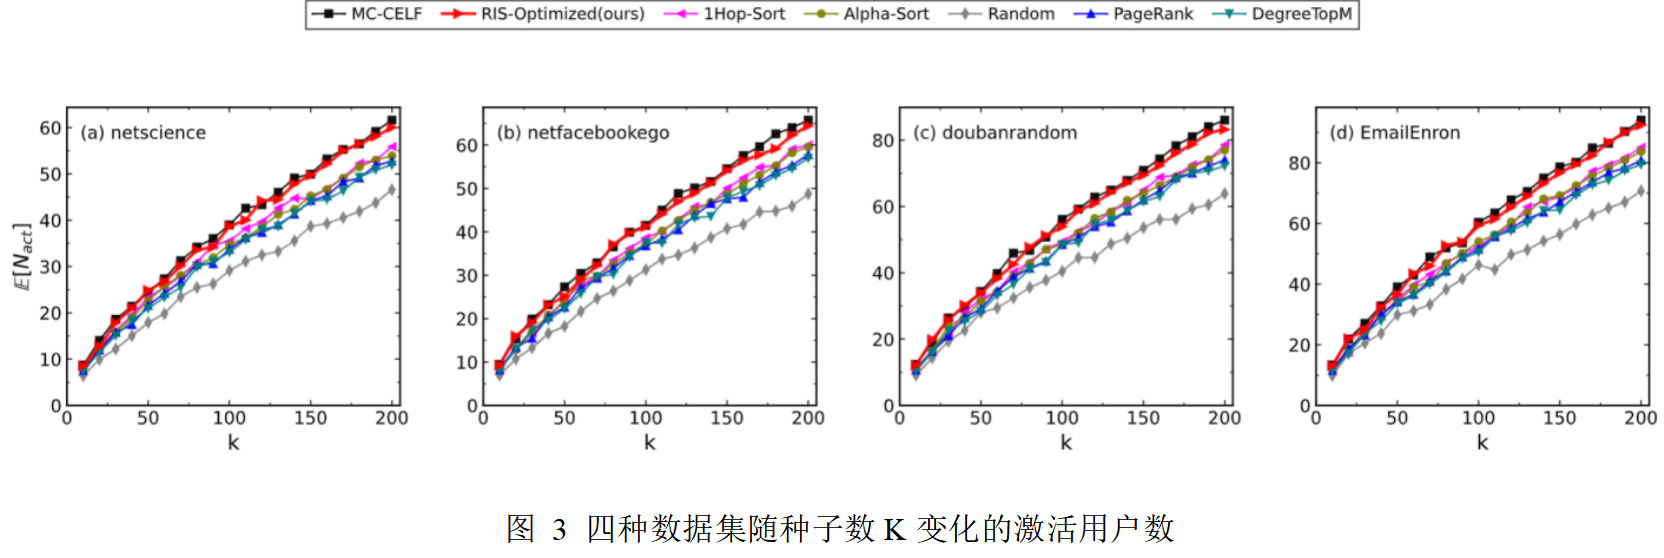
\includegraphics[width=\textwidth]{assets/fig_normal_spread}
  \caption{Adoption spread vs.\ seed budget $k$ under Scenario~I
    (Normal) across four datasets.
    \CIMRIS{} closely tracks the MC-CELF oracle;
    coupon-aware heuristics outperform topology-based baselines but
    fall behind \CIMRIS{} as $k$ grows.}
  \label{fig:normal_spread}
\end{figure*}

Fig.~\ref{fig:normal_redemp} reports total coupon redemptions under the
same conditions.
Under Scenario I, most nodes adopt at most one coupon, so redemption
curves closely mirror the adoption-spread curves.
\CIMRIS{} leads on both metrics, confirming that the benefits of global
spread optimization generalize beyond unique-user coverage.

\begin{figure*}[t]
  \centering
  %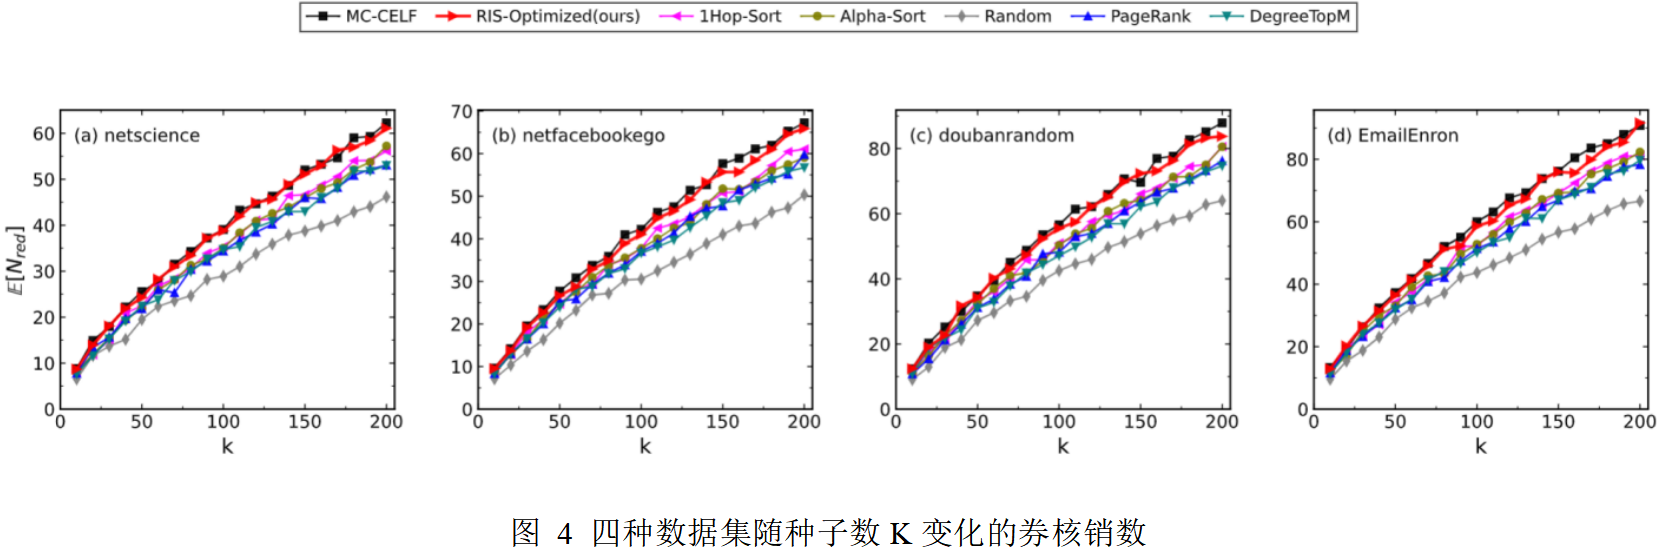
\includegraphics[width=\textwidth]{assets/fig_normal_redemption}
  \caption{Total coupon redemptions vs.\ $k$ under Scenario~I.
    Redemption curves mirror adoption-spread curves; \CIMRIS{} leads
    on both primary and secondary metrics.}
  \label{fig:normal_redemp}
\end{figure*}

\subsection{Model Validation: Coupon Influence vs.\ IC Baselines}
\label{sec:exp-ic}

Fig.~\ref{fig:ic_compare} isolates the comparison between \CIMRIS{} and
the two IC-model baselines.
\CIMRIS{} achieves substantially higher adoption spread across all four
datasets and all values of $k$.
The underperformance of IMM and OPIM is not attributable to algorithmic
weakness: both carry rigorous $(1{-}1/e{-}\epsilon)$-approximation
guarantees for the IC model.
The gap arises from \emph{structural model mismatch}.
IC optimization favors high-degree hubs, since broadcast diffusion
amplifies degree-centrality.
In coupon influence propagation, however, a node forwards to exactly one
neighbor; high out-degree confers no advantage over the single forward
it actually makes.
\CIMRIS{}, built around the actual single-path dynamics, correctly
identifies seeds that maximize adoption reach under coupon diffusion.
This result demonstrates that model fidelity-not just algorithmic
sophistication-is decisive for coupon campaign optimization.

\begin{figure*}[t]
  \centering
  %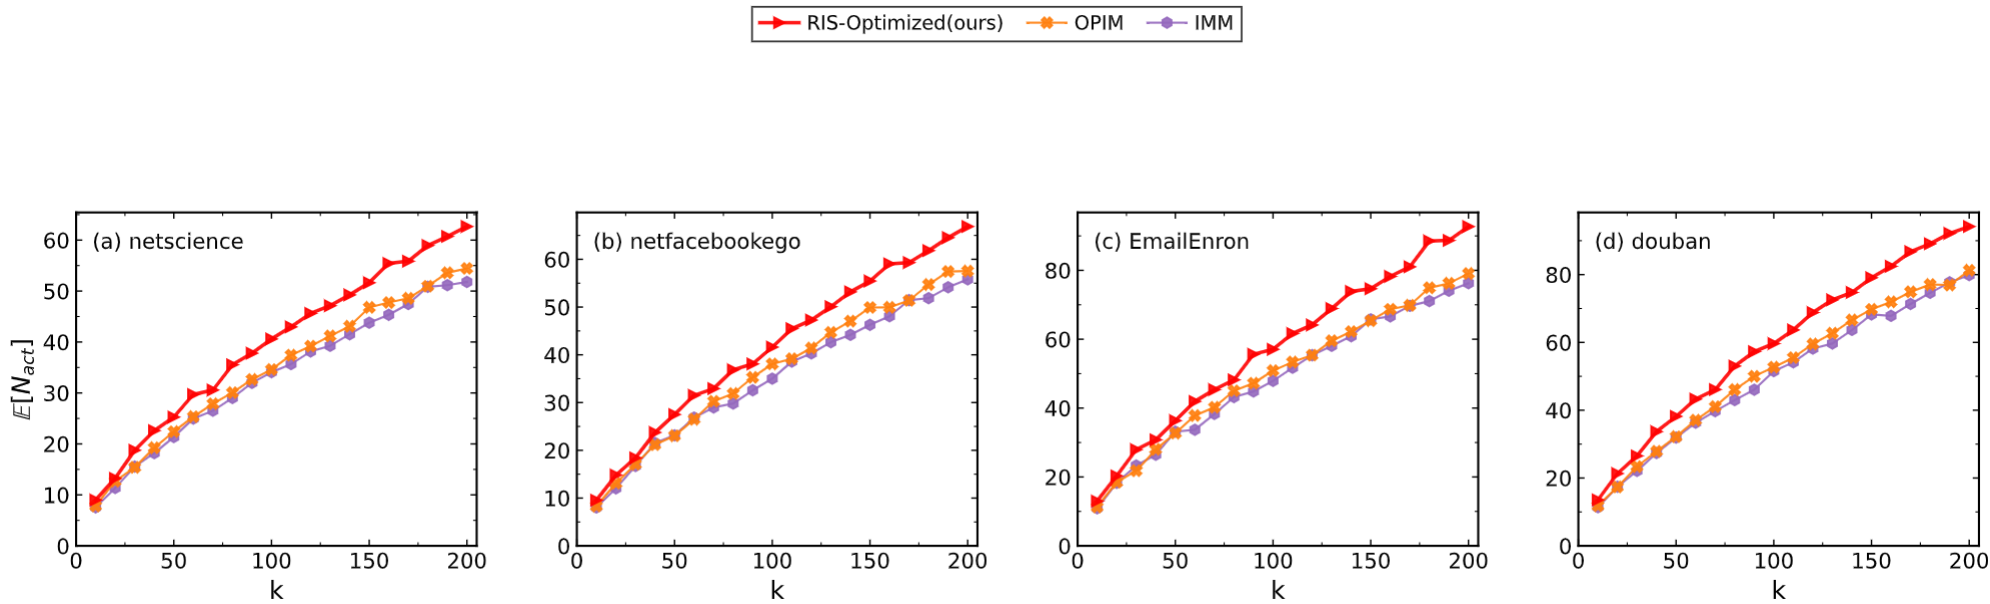
\includegraphics[width=\textwidth]{assets/fig_ic_comparison}
  \caption{Adoption spread of \CIMRIS{} vs.\ IC-model baselines (IMM,
    OPIM) under Scenario~I.
    Despite their theoretical guarantees for IC, both baselines
    consistently underperform because broadcast-influence optimization
    is structurally mismatched with non-replicable coupon propagation.}
  \label{fig:ic_compare}
\end{figure*}

\subsection{Effect of Diffusion Scenario}
\label{sec:exp-scenario}

Figs.~\ref{fig:high_fwd} and~\ref{fig:high_abs} show adoption spread
under Scenarios III and II, respectively.

\textbf{High Forwarding (Fig.~\ref{fig:high_fwd}).}
With $\E[p_u^t] \geq 0.88$, coupons trace long random walks before
terminating.
Absolute spread is lower than Scenario I because the per-step adoption
probability is tiny, but coupons travel far.
In this regime, global network structure dominates: seeds must be placed
where random walks tend to converge toward high-adoption regions.
The gap between \CIMRIS{} and all baselines widens relative to Scenario
I, reflecting how severely local heuristics fail when propagation is
long-range.

\begin{figure*}[t]
  \centering
  %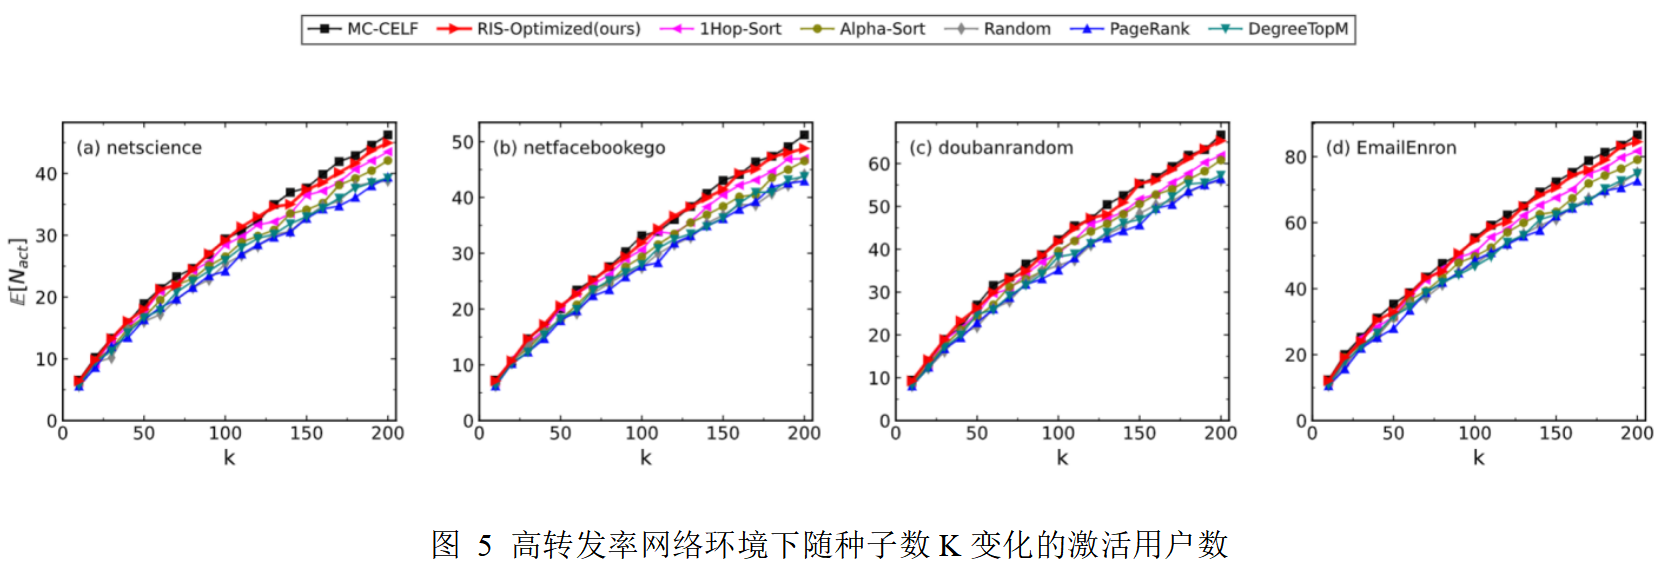
\includegraphics[width=\textwidth]{assets/fig_high_forwarding}
  \caption{Adoption spread vs.\ $k$ under Scenario~III (High
    Forwarding, $\E[p_u^t] \geq 0.88$).
    Long walks amplify the importance of global coverage; the gap
    between \CIMRIS{} and local heuristics widens.}
  \label{fig:high_fwd}
\end{figure*}

\textbf{High Absorption (Fig.~\ref{fig:high_abs}).}
With $\E[p_u^a + p_u^d] \approx 0.95$, coupons rarely propagate beyond
two hops.
Absolute spread is higher than Scenario I because immediate adoption is
likely.
Methods cluster more tightly because optimization reduces nearly to
covering disjoint one-hop neighborhoods-even simple heuristics
approximate this well.
\CIMRIS{} retains the lead, but the margin over 1 Hop-Sort and Alpha-Sort
narrows, consistent with the reduced role of long-range structure.

\begin{figure*}[t]
  \centering
  %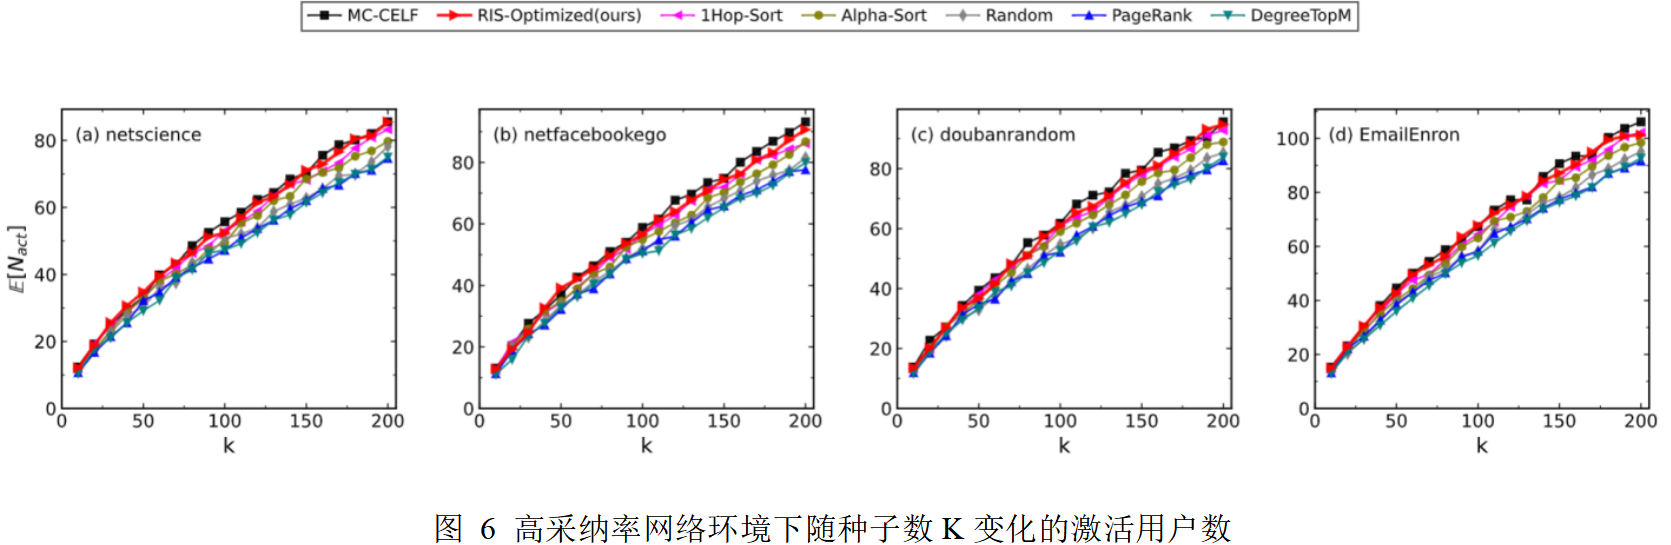
\includegraphics[width=\textwidth]{assets/fig_high_absorption}
  \caption{Adoption spread vs.\ $k$ under Scenario~II (High
    Absorption, $\E[p_u^a + p_u^d] \approx 0.95$).
    Short walks reduce the long-range optimization advantage; methods
    cluster tightly, yet \CIMRIS{} retains the lead.}
  \label{fig:high_abs}
\end{figure*}

\subsection{Running Time Analysis}
\label{sec:exp-runtime}

Fig.~\ref{fig:runtime} compares running time (ms, log scale) as a
function of $k$ across four datasets.
MC-CELF is omitted because it is prohibitively slow even on the
smallest graph.

Alpha-Sort and 1Hop-Sort complete in ${\sim}10^2$\,ms regardless of
$k$ or network size-both reduce to a single linear scan followed by
a sort.
PageRank requires iterative convergence and lands in the
$10^3$--$10^4$\,ms range on larger graphs.
\CIMRIS{} reaches $10^4$--$10^5$\,ms on EmailEnron, reflecting the
sampling budget required for the approximation guarantee; consistent
with the $O(k(k+\ell)(m+n)\log n/\epsilon^2)$ bound of
Theorem~\ref{thm:approx}, running time grows with both $k$ and
network size.

The results highlight a clear quality-efficiency trade-off.
Heuristics sacrifice spread quality, especially at large $k$ and under
High Forwarding, where long-range structure matters.
\CIMRIS{} pays a higher cost and in return matches the oracle.
For the intended use case-offline seed selection before a campaign
launches-this cost is well justified.

\begin{figure*}[t]
  \centering
  %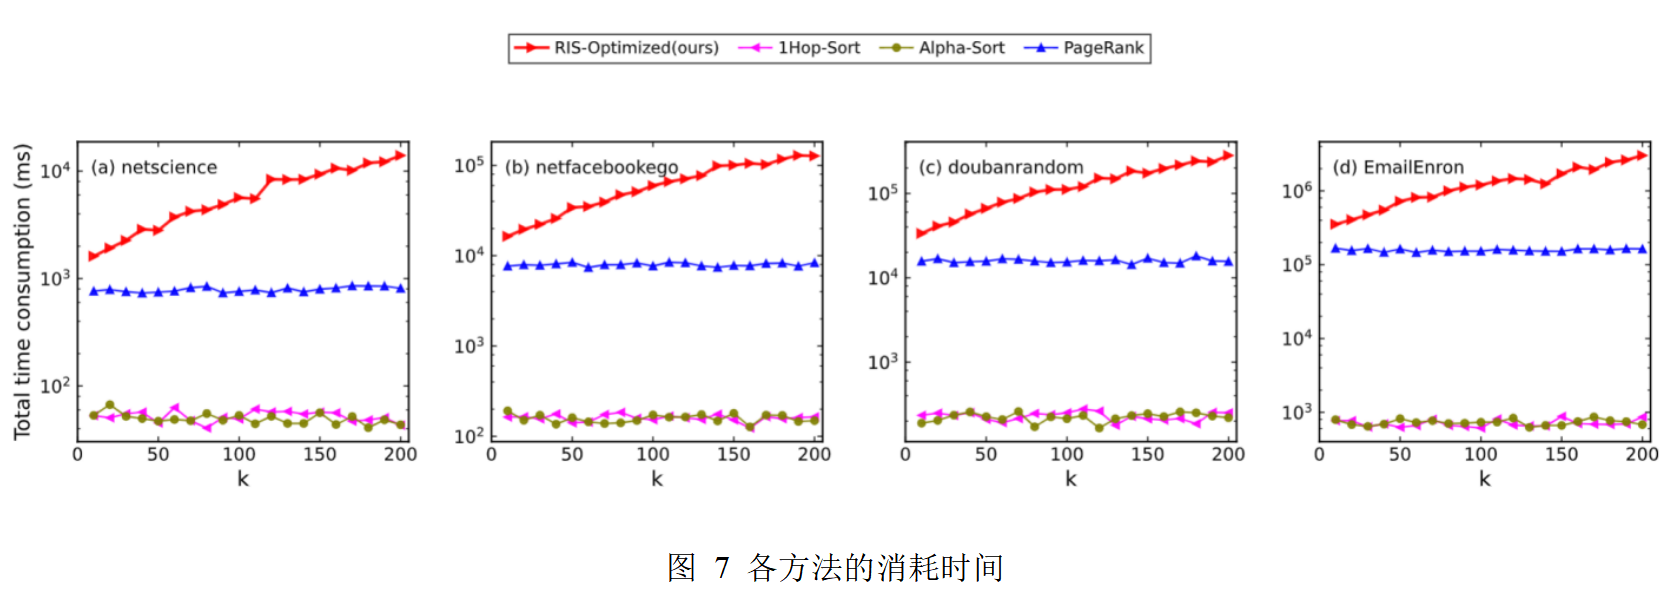
\includegraphics[width=\textwidth]{assets/fig_runtime}
  \caption{Running time (ms, log scale) vs.\ $k$ across four datasets.
    \CIMRIS{} is slower than heuristics due to $k$-joint RR-set
    sampling, but far faster than the MC-CELF oracle.}
  \label{fig:runtime}
\end{figure*}

%% ============================================================
%% 8. CONCLUSION
%% ============================================================
\section{Conclusion}
\label{sec:conclusion}

We introduced the coupon influence model and formalized CIM, capturing the
single-path, non-replicable dynamics of digital coupon campaigns that
fall outside the scope of classical IC/LT influence maximization.
The key structural distinction is twofold: the coupon moves to exactly
one neighbor at each step, and a user adopts only upon redemption
-not upon receipt.
We proved CIM is NP-hard and that adoption spread is monotone and
submodular, then bridged the gap between theory and practice by
developing $k$-joint RR sets with a provable unbiasedness lemma.
Our algorithm \CIMRIS{} runs in near-linear expected time with a
$(1/2{-}\epsilon)$-approximation guarantee.
Experiments on five real-world networks confirm that \CIMRIS{} matches
the Monte Carlo oracle while substantially outperforming both
model-mismatched IC baselines and coupon-aware heuristics-validating
that model fidelity is indispensable for optimizing non-replicable
coupon campaigns.

Several directions remain open.
First, extending the model to \emph{adaptive} seeding-where the
seed set of later stages depends on observed early adoptions-could
reduce budget waste in time-sensitive campaigns.
Second, the current model assumes the forwarding target is chosen
uniformly among neighbors; modeling biased forwarding
(e.g., users preferentially sharing with friends who would benefit
most) is a practically important extension.
Third, the connection between the coupon influence model and random walk theory
(e.g., hitting probabilities and cover times) may yield tighter bounds
on the expected RR-set size, improving the constant in the complexity
of \CIMRIS{}.

\begin{acks}
Acknowledgments omitted for anonymous review.
\end{acks}

\bibliographystyle{ACM-Reference-Format}
\bibliography{references}


\appendix
\section{Proof of Theorem~\ref{thm:nphard}}
\label{app:hardness}

We give a polynomial-time reduction from vertex cover in cubic
(3-regular) graphs~\cite{garey1976simplified}. An instance consists of
an undirected cubic graph $H=(V_H,E_H)$ and an integer $K$, and asks
whether a set of at most $K$ vertices meets every edge. We may restrict
to $1\leq K\leq |V_H|$, since the remaining budgets are trivial.

\paragraph{Construction.}
Create a directed graph $G=(V,E)$ with
\[
  V=A\cup B_H,\qquad
  A=\{a_x:x\in V_H\},\quad B_H=\{b_e:e\in E_H\}.
\]
For each incidence $x\in e$, add the arc $(a_x,b_e)$.
At each $a_x$, set
\[
  (p_{a_x}^a,p_{a_x}^d,p_{a_x}^t)=(1/2,0,1/2),
  \qquad p(a_x,b_e)=1/3\quad(x\in e).
\]
At each $b_e$, set
$(p_{b_e}^a,p_{b_e}^d,p_{b_e}^t)=(1/4,3/4,0)$.
The coupon budget is $k=K$, and every node in $V$ is eligible as a
seed. The graph is acyclic with two layers. Conditional forwarding
probabilities sum to one at every node with out-neighbors, and the
termination probability is at least $1/2$ everywhere. Thus the
construction satisfies the model of Section~\ref{sec:model}, including
independence across coupons. It has $|V_H|+|E_H|$ nodes and $2|E_H|$
arcs, and all probabilities have constant-size rational encodings.

\paragraph{Eliminating seeds in the second layer.}
Consider any seed set $S\subseteq V$ with $|S|=K$ that contains a node
$b_e$. Since $K\leq |A|$, some $a_x\in A$ is unselected. The coupon
seeded at $b_e$ can only be consumed there, with probability $1/4$;
removing this seed therefore decreases $\sigma$ by at most $1/4$.
No node has an arc into $a_x$, so no other seed's coupon can be
consumed at $a_x$. Adding $a_x$ increases $\sigma$ by at least its
self-consumption probability $1/2$. Thus replacing $b_e$ by $a_x$
strictly improves the objective. Repeating this replacement produces
a $K$-element subset of $A$ with no smaller spread. In particular,
every optimal seed set is contained in $A$.

\paragraph{Objective value.}
For a seed $a_x$, the only nonzero eventual-consumption probabilities
are
\[
  q_{a_x,a_x}=\frac12,\qquad
  q_{a_x,b_e}=\frac12\cdot\frac13\cdot\frac14=\frac1{24}
  \quad(x\in e).
\]
Let $S\subseteq A$ have size $K$, and let $c_e(S)\in\{0,1,2\}$ be
the number of endpoints of $e$ whose corresponding nodes belong to
$S$. Independence of the coupons gives
\[
  \sigma(S)=\frac K2+
    \sum_{e\in E_H}\left[1-\left(1-\frac1{24}\right)^{c_e(S)}\right].
\]
For $i\in\{0,1,2\}$, let $n_i$ count the edges with $c_e(S)=i$.
Since every vertex of $H$ has degree three,
\[
  n_0+n_1+n_2=|E_H|,\qquad n_1+2n_2=3K.
\]
Consequently,
\begin{align*}
  \sigma(S)
    &=\frac K2+\frac{n_1}{24}
      +n_2\left(\frac2{24}-\frac1{576}\right)\\
    &=\frac K2+\frac{3K}{24}-\frac{n_2}{576}\\
    &=\frac K2+\frac{3K}{24}
      -\frac{3K-|E_H|+n_0}{576}.
\end{align*}

\paragraph{Correctness of the reduction.}
Set
\[
  B=\frac K2+\frac{3K}{24}-\frac{3K-|E_H|}{576}.
\]
If $H$ has a vertex cover of size at most $K$, extend it to exactly
$K$ vertices and select the corresponding nodes of $A$. Every edge
then has a selected endpoint, so $n_0=0$ and $\sigma(S)=B$.
Conversely, suppose some $K$-node seed set has spread at least $B$.
The replacement argument yields a set $S\subseteq A$ of the same
size with spread at least $B$. Its objective is $B-n_0/576$, which
forces $n_0=0$. The corresponding vertices therefore cover $H$.
The rational threshold $B$ has polynomial encoding length, so this
establishes a polynomial-time reduction and proves NP-hardness.

\end{document}
